\begingroup
\definecolor{gatecore}{RGB}{30,106,79}
\definecolor{gatetube}{RGB}{236,246,240}
\definecolor{gatechamber}{RGB}{235,242,252}
\definecolor{gatehigh}{RGB}{250,226,211}
\definecolor{gatepath}{RGB}{29,75,132}
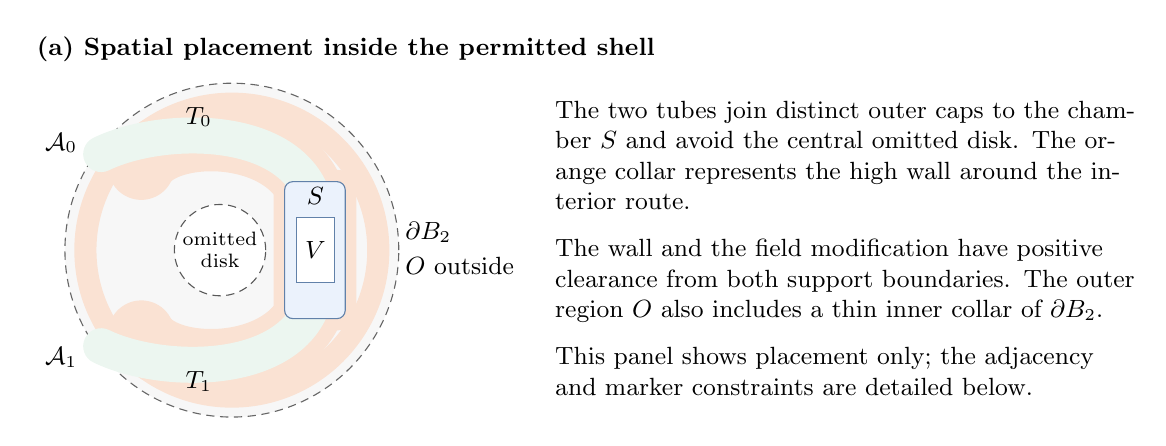
\begin{tikzpicture}[x=1cm,y=1cm,font=\small,
  cheap/.style={draw=gatetube,line width=13pt,line cap=round,line join=round},
  wall/.style={draw=gatehigh,line width=24pt,line cap=round,line join=round}]
  \node[anchor=west,font=\small\bfseries] at (0,4.90)
    {(a) Spatial placement inside the permitted shell};
  \fill[black!3] (2.60,2.35) circle (2.12);
  \draw[black!60,densely dashed] (2.60,2.35) circle (2.12);
  \draw[gatehigh,line width=8pt] (2.60,2.35) circle (1.86);
  \draw[wall] (1.45,3.41) .. controls (1.70,3.94) and (3.37,3.97) .. (3.65,2.96);
  \draw[wall] (1.45,1.29) .. controls (1.70,.76) and (3.37,.73) .. (3.65,1.74);
  \filldraw[fill=gatehigh,draw=none,rounded corners=7pt]
    (3.13,1.33) rectangle (4.18,3.37);
  \draw[cheap] (.94,3.57) .. controls (1.70,3.94) and (3.37,3.97) .. (3.65,2.96);
  \draw[cheap] (.94,1.13) .. controls (1.70,.76) and (3.37,.73) .. (3.65,1.74);
  \filldraw[fill=gatechamber,draw=gatepath!70,rounded corners=3pt]
    (3.27,1.48) rectangle (4.04,3.22);
  \filldraw[fill=white,draw=gatepath!70]
    (3.42,1.94) rectangle (3.90,2.76);
  \node at (3.66,2.35) {$V$};
  \node at (3.66,3.04) {$S$};
  \filldraw[fill=white,draw=black!65,densely dashed]
    (2.45,2.35) circle (.58);
  \node[align=center,font=\scriptsize] at (2.45,2.35)
    {omitted\\disk};
  \node[anchor=east] at (.76,3.71) {$\mathcal A_0$};
  \node[anchor=east] at (.76,.99) {$\mathcal A_1$};
  \node at (2.18,4.04) {$T_0$};
  \node at (2.18,.68) {$T_1$};
  \node[anchor=west] at (4.68,2.58) {$\partial B_2$};
  \node[anchor=west] at (4.68,2.15) {$O$ outside};
  \node[anchor=north west,align=left,text width=7.4cm,inner sep=0pt]
    at (6.70,4.25) {The two tubes join distinct outer caps to the
      chamber $S$ and avoid the central omitted disk.  The orange
      collar represents the high wall around the interior route.
      \par\medskip
      The wall and the field modification have positive clearance
      from both support boundaries.  The outer region $O$ also
      includes a thin inner collar of $\partial B_2$.
      \par\medskip
      This panel shows placement only; the adjacency and marker
      constraints are detailed below.};
\end{tikzpicture}

\par\medskip
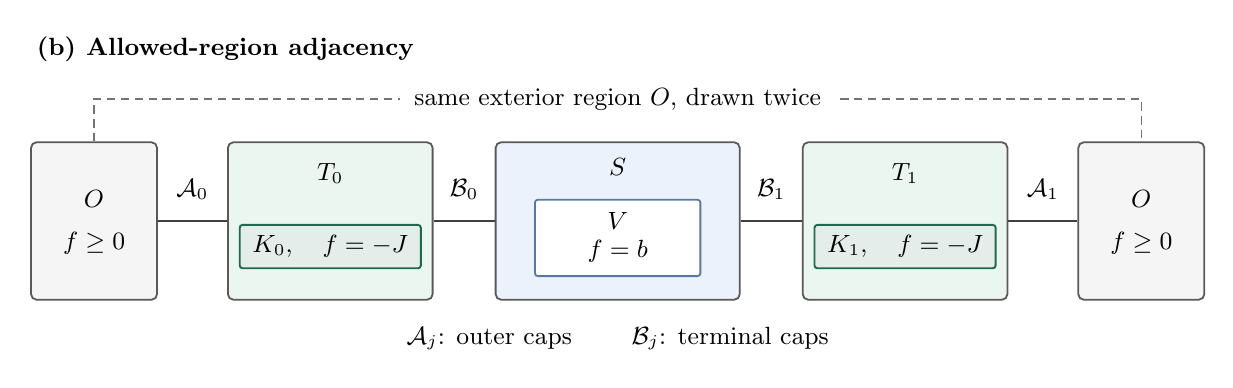
\begin{tikzpicture}[x=1cm,y=1cm,font=\small,
  region/.style={draw=black!65,line width=.65pt,rounded corners=2pt,
                 minimum height=2cm,inner sep=0pt},
  caplink/.style={draw=black!75,line width=.8pt}]
  \node[anchor=west,font=\small\bfseries] at (0,3.18)
    {(b) Allowed-region adjacency};

  \node[region,fill=black!4,minimum width=1.6cm] (outerleft) at (.85,1) {};
  \node[region,fill=gatetube,minimum width=2.6cm] (tubezero) at (3.85,1) {};
  \node[region,fill=gatechamber,minimum width=3.1cm] (chamber) at (7.5,1) {};
  \node[region,fill=gatetube,minimum width=2.6cm] (tubeone) at (11.15,1) {};
  \node[region,fill=black!4,minimum width=1.6cm] (outerright) at (14.15,1) {};

  \draw[densely dashed,black!55,line width=.55pt]
    (outerleft.north) -- (.85,2.55) -- (14.15,2.55) -- (outerright.north);
  \node[fill=white,inner xsep=5pt,inner ysep=2pt] at (7.5,2.55)
    {same exterior region $O$, drawn twice};

  \draw[caplink] (outerleft.east) --
    node[above=4pt] {$\mathcal A_0$} (tubezero.west);
  \draw[caplink] (tubezero.east) --
    node[above=4pt] {$\mathcal B_0$} (chamber.west);
  \draw[caplink] (chamber.east) --
    node[above=4pt] {$\mathcal B_1$} (tubeone.west);
  \draw[caplink] (tubeone.east) --
    node[above=4pt] {$\mathcal A_1$} (outerright.west);

  \node at (.85,1.28) {$O$};
  \node at (.85,.72) {$f\geq0$};
  \node at (14.15,1.28) {$O$};
  \node at (14.15,.72) {$f\geq0$};
  \node at (3.85,1.60) {$T_0$};
  \node at (11.15,1.60) {$T_1$};
  \node at (7.5,1.68) {$S$};

  \filldraw[fill=gatecore!12,draw=gatecore,line width=.7pt,rounded corners=1pt]
    (2.70,.40) rectangle (5.00,.95);
  \node at (3.85,.675) {$K_0,\quad f=-J$};
  \filldraw[fill=gatecore!12,draw=gatecore,line width=.7pt,rounded corners=1pt]
    (10.00,.40) rectangle (12.30,.95);
  \node at (11.15,.675) {$K_1,\quad f=-J$};
  \filldraw[fill=white,draw=gatepath!75,line width=.65pt,rounded corners=1pt]
    (6.45,.30) rectangle (8.55,1.27);
  \node[align=center] at (7.5,.79) {$V$\\[-1pt]$f=b$};

  \node[anchor=north] at (7.5,-.22)
    {$\mathcal A_j$: outer caps \qquad $\mathcal B_j$: terminal caps};
\end{tikzpicture}

\par\medskip

\begin{tikzpicture}[x=1cm,y=1cm,font=\small,
  transit/.style={draw=gatepath,line width=1.05pt,-{Stealth[length=2mm]}}]
  \node[anchor=west,font=\small\bfseries] at (0,3.75)
    {(c) A transverse marker forces access to the core};

  \fill[gatetube] (.35,.25) rectangle (9.15,2.95);
  \fill[gatehigh] (4.10,.25) rectangle (5.80,2.95);
  \node[anchor=west] at (.48,3.20) {$T_j$};
  \draw[decorate,decoration={brace,amplitude=3pt},black!65]
    (4.10,3.06) -- (5.80,3.06);
  \node[anchor=south] at (4.95,3.15) {marker slab};

  \filldraw[fill=white,draw=gatecore!65,densely dashed,line width=.65pt,
            rounded corners=3pt]
    (.82,1.05) rectangle (8.68,2.10);
  \filldraw[fill=gatecore!14,draw=gatecore,line width=.8pt,
            rounded corners=1pt]
    (1.00,1.38) rectangle (8.50,1.76);
  \node at (2.40,1.57) {$K_j,\quad f=-J$};
  \node at (4.95,2.53) {$f=H$};
  \node at (4.95,.63) {$f=H$};

  \draw[black!55,line width=.55pt] (4.10,.25) -- (4.10,2.95);
  \draw[black!55,line width=.55pt] (5.80,.25) -- (5.80,2.95);
  \draw[black!65,line width=.7pt,rounded corners=2pt]
    (.35,.25) rectangle (9.15,2.95);

  \draw[transit] (.65,2.43)
    .. controls (2.35,2.56) and (3.32,1.98) .. (4.30,1.95)
    -- (5.70,1.95)
    .. controls (6.80,1.95) and (7.48,2.46) .. (8.85,2.43);
  \fill[gatepath] (4.55,1.95) circle (1.7pt);
  \node[anchor=south east,inner sep=2pt,text=gatepath] at (4.50,2.02) {$p_j$};
  \draw[gatecore,line width=.65pt,-{Stealth[length=1.4mm]}]
    (4.55,1.91) -- (4.55,1.61);
  \node[anchor=north west,inner sep=0pt] at (.84,.91)
    {core's $\rho$-collar};
  \draw[black!60,line width=.45pt] (2.47,.89) -- (2.88,1.05);

  \node[anchor=north west,align=left,text width=5.0cm,inner sep=0pt]
    at (9.72,2.96) {A complete transit with $D^f$-length at most $B_0$
      must enter the $\rho$-collar, since
      \[
        e^{\xi H}m_*w>2B_0.
      \]
      From such a point $p_j$, the cheap core and terminal hop give
      \[
        D^f(p_j,z_j;\text{local collar})<e.
      \]};
\end{tikzpicture}
\endgroup
